\documentclass[10pt,professionalfonts]{beamer}
\usepackage[utf8]{inputenc}
\usepackage[T1]{fontenc}
\usepackage[english]{babel}
\usepackage{unicode}
\usepackage{booktabs}
\usepackage{lmodern,sfmath}
\DeclareUnicodeCharacter{2713}{\checkmark}
\usepackage{animate}
\usepackage{graphicx}
\graphicspath{{graphics/}}

\makeatletter
\usetheme{CambridgeUS}%<<<
\definecolor{bleu}{rgb}{.1,.4,.6}%1a6699
\definecolor{rouge}{rgb}{.6,.1,.15}%991a26

\mode<presentation>{
\setbeamercolor{structure}{fg=rouge!80}
\setbeamercolor{palette primary}{fg=white,bg=rouge}
\setbeamercolor{palette secondary}{fg=white,bg=rouge!90}
\setbeamercolor{palette tertiary}{fg=white,bg=rouge!80}
\setbeamercolor{palette quaternary}{fg=white,bg=rouge!70}
\setbeamercolor{title}{fg=white,bg=bleu!60}
\setbeamercolor{section in head/foot}{fg=white,bg=bleu!90}
\setbeamercolor{subsection in head/foot}{fg=white,bg=bleu}
\setbeamercolor{frametitle}{fg=white,bg=bleu!80}
\setbeamercolor{titlelike}{parent=palette quaternary}
\setbeamercolor{block title}{fg=white,bg=bleu!80}
\setbeamercolor{block body}{fg=black,bg=bleu!20}
% couleurs perso pour ce qui suit
\setbeamercolor{strong}{fg=rouge}
\setbeamercolor{emph}{fg=bleu}
\setbeamercolor{table head}{fg=white,bg=bleu!80}
\setbeamercolor{table odd}{bg=bleu!20}
\setbeamercolor{table even}{bg=bleu!10}
}
\useinnertheme{rectangles}
\setbeamertemplate{blocks}[default]
\setbeamertemplate{title page}[default][rounded=false,shadow=false]
\setbeamertemplate{navigation symbols}{}


\defbeamertemplate{itemize item}{exemple}{{\color{bleu}$\rhd$}}
\defbeamertemplate{itemize subitem}{exemple}{{\color{bleu}$\rhd$}}
\newenvironment<>{exemple}{\begin{actionenv}%
  \ifnum\@itemdepth = 0 \setbeamertemplate{itemize item}[exemple]%
  \else \setbeamertemplate{itemize subitem}[exemple]\fi
  \begin{itemize}\item}%
  {\end{itemize}\end{actionenv}}
%>>>
\def\strong#1{{\usebeamercolor{strong}\textcolor{fg}{\textbf{#1}}}}
\def\imp#1{{\usebeamercolor{emph}\textcolor{fg}{\emph{#1}}}}
% Section frames%<<<
\let\oldsection\section
\newenvironment<>{sectionblock}[1]{%
  \begin{actionenv}#2\def\insertblocktitle{#1}%
  \mode<presentation>{%
    \setbeamercolor{block body}{fg=white,bg=rouge!90}
  }\usebeamertemplate{block begin}}%
{\par\usebeamertemplate{block end}\end{actionenv}}%
\newenvironment<>{subsectionblock}[1]{%
  \begin{actionenv}#2\def\insertblocktitle{#1}%
    \mode<presentation>{%
            \setbeamercolor{block body}{fg=white,bg=rouge!80}
    }\usebeamertemplate{block begin}}%
{\par\usebeamertemplate{block end}\end{actionenv}}%

\newif\if@sectionframe@cnt \@sectionframe@cnttrue
\def\sectionframe{\@ifstar
  {\@sectionframe@cntfalse\@sectionframe}%
  {\@sectionframe@cnttrue \@sectionframe}%
}
\def\thesection{\@Roman\c@section}
\def\thesubsection{\@arabic\c@subsection}
\def\@sectionframe#1{%
  \def\insertsectionhead{}\def\insertsubsectionhead{}\begin{frame}%
  \begin{center}\begin{sectionblock}{}\hfil\Large\strut
  \if@sectionframe@cnt \stepcounter{section}\thesection~--~\fi
  #1\end{sectionblock}
  \addtocounter{section}\m@ne
  \end{center}\end{frame}\section{#1}}
\def\subsectionframe#1{%
  \def\insertsubsectionhead{}\begin{frame}\begin{center}
  \begin{sectionblock}{}\hfil\Large\strut\insertsectionhead
  \end{sectionblock}
  \begin{subsectionblock}{}%
  \stepcounter{subsection}
  \hfil \large \thesubsection. #1\end{subsectionblock}
  \addtocounter{subsection}\m@ne
\end{center}\end{frame}\subsection{#1}}
%>>>
% Autoriser les blocs sans titre%<<<
\setbeamertemplate{block begin}{\par\medskip
 \ifx\insertblocktitle\empty\else
 \par\vskip\medskipamount%
  \begin{beamercolorbox}[colsep*=.75ex]{block title}
    \usebeamerfont*{block title}\insertblocktitle%
  \end{beamercolorbox}%
 {\parskip0pt\par}%
  \ifbeamercolorempty[bg]{block title}
  {}
  {\ifbeamercolorempty[bg]{block body}{}{\nointerlineskip\vskip-0.5pt}}%
 \fi
  \usebeamerfont{block body}%
  \begin{beamercolorbox}[colsep*=.75ex,vmode]{block body}%
    \ifbeamercolorempty[bg]{block body}{\vskip-.25ex}{\vskip-.75ex}\vbox{}%
}%>>>
\RequirePackage{colortbl}
% Playing with colortbl%<<<
% definining \tablecolor: the default color for a table
\let\orig@CT@setup\CT@setup
\let\CT@tablecolor\@empty
\let\CT@tablefg\@empty
\let\CT@rowfg\@empty
%
\def\tablecolor#1{\def\CT@tablecolor{#1}}
% defining \tablecoloralt: alternating colors for table rows
\let\CT@tablecoloraltI\@empty
\let\CT@tablecoloraltII\@empty
\def\tablecoloralt#1#2{\def\CT@tablecoloraltI{#1}\def\CT@tablecoloraltII{#2}}
\def\tablefg#1{\noalign{\gdef\CT@tablefg{#1}}}
\def\rowfg#1{\noalign{\gdef\CT@rowfg{#1}}}
% modifying start/save macros%<<<
\def\CT@start{%
  \let\CT@arc@save\CT@arc@
  \let\CT@drsc@save\CT@drsc@
  \let\CT@row@color@save\CT@row@color
  \let\CT@cell@color@save\CT@cell@color
  \let\CT@tablecoloraltI@save\CT@tablecoloraltI
  \let\CT@tablecoloraltII@save\CT@tablecoloraltII
  \def\CT@tablerowsave{\the\tablerow}\tablerow 0
  \def\+{\noalign{\CT@samerow}}%
  \global\let\CT@cell@color\relax}
\def\CT@end{%
  \global\let\CT@arc@\CT@arc@save
  \global\let\CT@drsc@\CT@drsc@save
  \global\let\CT@row@color\CT@row@color@save
  \global\let\CT@cell@color\CT@cell@color@save
  \let\CT@tablecoloraltI\CT@tablecoloraltI@save
  \let\CT@tablecoloraltII\CT@tablecoloraltII@save
  \expandafter \tablerow \CT@tablerowsave
}%>>>
\newcount\tablerow \def\CT@samerow{\global\advance\tablerow -1}
\CT@everycr{\noalign{\global\let\CT@row@color\relax
  \global\let\CT@rowfg\@empty
  \global\advance\tablerow 1}\the\everycr}
\def\CT@setup{\orig@CT@setup
  \ifx\CT@tablecoloraltI\@empty
    \ifx\CT@tablecolor\@empty\else\CT@color{\CT@tablecolor}\fi
  \else \ifodd\tablerow \CT@color{\CT@tablecoloraltI}%
    \else \CT@color{\CT@tablecoloraltII}\fi\fi
  \ifx\CT@rowfg\@empty \else
    \global\setbox\z@ \hbox{{\color{\CT@rowfg}\unhbox \z@}}\fi
  \ifx\CT@tablefg\@empty \else
    \global\setbox\z@ \hbox{{\color{\CT@tablefg}\unhbox \z@}}\fi
} % >>>
% Tableaux (utilise colortbl)%<<<
\newenvironment<>{tableau}[1]{\begin{actionenv}%
  \usebeamercolor{table head}
  \usebeamercolor{table odd}\usebeamercolor{table even}
  \def\entete{\+\rowcolor{table head.bg}\rowfg{table head.fg}}%
  \def\arraystretch{1.2}
  \tablecoloralt{table odd.bg}{table even.bg}\begin{tabular}{#1}}
  {\end{tabular}\end{actionenv}}
%>>>
% Macros perso
\def\abs#1{\left|#1\right|}
\def\pa#1{\left(#1\right)}
\def\acco#1{\left\{#1\right\}}
\def\bib#1{{\usebeamercolor{emph}\textcolor{fg}{~[#1]}}}
\def\F{\mathbb{F}}
\def\prob{\mathcal{P}}

\makeatother

\begin{document}
\title[Diversity and Transparency for ECC]{Diversity and Transparency for ECC}
\author[J.-P. Flori]{Jean-Pierre Flori, Jérôme Plût, Jean-René
Reinhard, and Martin Ekerå}
\institute[ANSSI]{ANSSI and NCSA/SW}
\date{June 11, 2015}

\begin{frame}<handout:0> \titlepage
\end{frame}

\sectionframe{Standardization}

\begin{frame}\frametitle{Need for standardization?}
\begin{block}{}
\strong{In general,} the group of rational points of an elliptic curve
behaves as a ``generic group'':
the DLOG problem has \strong{exponential} complexity, provided:
\end{block}
\begin{itemize}
\item The curve cardinality includes a \imp{large prime factor} $q$.
\begin{itemize}
\item Solution: use curves with (almost) prime cardinality.
\end{itemize}
\item The DLOG problem can not be transferred into \imp{weaker} groups.
\begin{itemize}
\item Solution: avoid weak curves.
\end{itemize}
\end{itemize}
\begin{block}{}
Applying these solutions is \strong{computationally expensive}:
curves can not be generated on demand.
\end{block}
\end{frame}

\begin{frame}\frametitle{Standardized curves}
\begin{center}\begin{tableau}{lcll}
\entete Year & & Curves & Sizes \\
2000 & 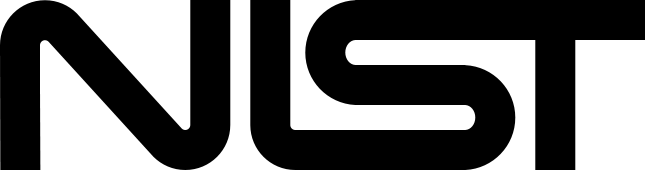
\includegraphics[height=1em]{nist} & NIST & 192, 224, 256, 384, 521\\
2005 & 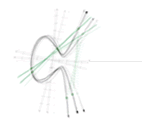
\includegraphics[height=2em]{brainpool} & Brainpool & 160, 192, 224, 256, 320, 384, 512\\
2010 & 
\includegraphics[height=2em]{oscca} & OSCCA & 256 \\
2011 & 
\includegraphics[height=2em]{anssi} & ANSSI & 256 \\
\end{tableau}\end{center}
\begin{itemize}
\item Plus a few academic propositions (Curve25519/41417, NUMS, Ed448-Goldilocks, \ldots).
\end{itemize}
\end{frame}

\begin{frame}\frametitle{Need for a second round?}
The first curves were standardized in years 2000
when:
\begin{itemize}
\item it was possible to find curves with prime cardinality
(SEA algorithm);
\item weak classes of curves were identified.
\end{itemize}
\begin{block}{}
We think that these curves are still secure\ldots
\end{block}
\ldots but new concerns emerged since then:
\begin{itemize}
\item what about the generation process?
(is there some hidden secret vulnerability?)
\item what about side-channel attacks?
\item what about scientific progess in related domains (e.g. DLOG in finite fields)?
\end{itemize}
\begin{block}{}
It is a good time to standardize new curves.
\end{block}
\end{frame}

\sectionframe{Security}

\begin{frame}\frametitle{Five classes of criteria}
\begin{enumerate}
\item The \strong{DLOG} problem should be hard.
\item Implementations should be \strong{safe} (e.g. resist \imp{side-channel attacks}).
\item The curve should exhibit no \strong{particularities}.
\item Implementations can be \strong{optimized}.
\item (The curve exhibits \strong{interesting} properties.)
\end{enumerate}
\begin{block}{Tradeoffs}
Some conditions are \strong{incompatible}:
this is a good reason to standardize \imp{different} (families of) curves.
\end{block}
\begin{block}{Base field}
We only deal with \imp{prime base fields} as we think that \imp{extension fields}
introduce more vulnerabilities without valuable properties.
\end{block}
\end{frame}

\subsection{DLOG problem difficulty}

\begin{frame}\frametitle{DLOG problem difficulty}
\begin{itemize}
\item \strong{Large prime subgroup}:
Attacks with complexity~$O(√q)$ exist where $q$ is the largest prime factor of $N$.
\begin{block}{}
It is mandatory that:
\begin{itemize}
\item \imp{$q ≈ N$} ($\prob ≈ \frac{1}{\log p}$, costly).
\item At best \imp{$q = N$} (\emph{no complete addition law!}).
\end{itemize}
\end{block}
\bigskip
\item \strong{Weak curves}:
For some curves the DLOG problem can be transferred into a weaker finite field.
\begin{block}{}
It is mandatory that:
\begin{itemize}
\item \imp{$Δ ≠ 0$} ($\prob ≈ 1$, free);
\item \imp{$N ≠ p$} ($\prob ≈ 1$, free);
\item the \imp{embedding degree} must be large ($\prob ≈ 1$, costly).
\end{itemize}
\end{block}
\end{itemize}
\end{frame}

\subsection{Safe implementation}

\begin{frame}\frametitle{Safe implementation}
\begin{block}{}
Even though the DLOG problem is \imp{hard} on the curve,
implementations might \strong{leak} information.
\end{block}
Example: scalar multiplication using naive ``double-and-add'' algorithm.
\begin{center}
\includegraphics[width=24em,height=8em]{spa.pdf}
\hskip 1.2em
 \begin{tabular}{|p{1.45em}|p{1.45em}|p{1.45em}|p{1.45em}|p{1.45em}|p{1.45em}|p{1.45em}|p{1.45em}|} 
 \hline
 D&A&D&D& D&A&D&A\\
 \hline
 \multicolumn{2}{|c|}{1} &
 \vrule width 0pt height 2ex
 0 & 0 & \multicolumn{2}{|c|}{1} & \multicolumn{2}{|c|}{1} \\
 \hline
 \end{tabular}
\end{center}
\end{frame}

\begin{frame}\frametitle{Classical countermeasures}
\begin{itemize}
\item Against \strong{simple} attacks:
avoid branching depending on secret elements.
\begin{itemize}
\item ``double-and-add'' always;
\item Montgomery ladder.
\end{itemize}
\item Against \strong{differential} attacks:
avoid using secrets elements repeatedly.
\begin{itemize}
\item secret \imp{masking};
\item curve \imp{masking};
\item point \imp{masking}.
\end{itemize}
\end{itemize}
\medskip
\begin{block}{}
This is not enough: information can still \strong{leak}!
\end{block}
\end{frame}

\begin{frame}\frametitle{Further countermeasures}
\begin{block}{Masking inefficiency}
Avoid base field with \imp{special prime} cardinality (\emph{no fast reduction!}).
\end{block}
\begin{block}{Exceptional cases}
Use a curve with a \imp{complete} addition law (\emph{no prime cardinality!}).
\end{block}
\begin{block}{Special points}
Ensure no points with a \imp{zero coordinate} exist (\emph{no complete addition law!}).
\end{block}
\end{frame}

\begin{frame}\frametitle{Misbehavior resistance}
\begin{block}{Subgroup attacks}
Ensure no \imp{small subgroups} exist ($\prob = 1$ if $N$ is prime, \emph{no complete addition law!}).
\end{block}
\medskip
\begin{block}{Twist security}
The \imp{twist} has prime cardinality (\strong{$\prob ≈ \frac{1}{\log p}$}).
\end{block}
\end{frame}

\subsection{Genericity}

\begin{frame}\frametitle{Resist attacks to come?}
\begin{itemize}
\item What if we don't know all classes of \strong{weak} curves?
\item Avoid producing too ``\imp{special}'' curves!
\item Verify properties satisfied with~\strong{$\prob ≈ 1$} in the sense of the DLOG problem difficulty.
\item In particular, some \strong{numbers attached to the curve} should be ``\imp{large enough}''.
\end{itemize}
\end{frame}

\begin{frame}\frametitle{Numbers attached to a curve}
\begin{block}{Discriminant of the endomorphism ring}
In general, the \imp{discriminant} satisfies $\abs{D_E} ≈ p$ ;
therefore, $\abs{D_{E}} ≥ √p$ with~$\prob ≈ 1-O(1/√p)$ (\emph{no pairings, no fast endomorphism!}).
\end{block}
\begin{block}{Class number friability}
In general, the \imp{class number} $h_E$ has at least a prime divisor~$≥ (\log p)^{O(1)}$.
\end{block}
\begin{block}{Embedding degree}
The \imp{embedding degree} is~$≥ p^{1/4}$
with~$\prob ≥ 1-1/√p$ (\emph{no pairings!}).
\end{block}
\end{frame}

\begin{frame}\frametitle{Numbers attached to a curve (II)}
\begin{block}{Twist cardinality}
In general, the \imp{twist cardinality} $N'$ has at least
a prime divisor of polynomial size in~$p$.
\end{block}
\begin{block}{DLOG in the base field}
\begin{itemize}
\item The base field cardinality $p$ should be \strong{pseudo-random}
(\emph{no fast reduction!}).
\item $p-1$ has a prime divisor $≥ (\log p)^2$ with $\prob ≥ 1-1/√p$.
\end{itemize}
\end{block}
\end{frame}

\begin{frame}\frametitle{Summary}
\begin{center}\begin{tableau}{*{5}{l}}
\entete       & NIST & Brainpool & ANSSI & OSCCA\\
$N$ prime   &  ✓   & ✓         & ✓     & ✓   \\
$p$ ordinary &      & ✓         & ✓     & ✓   \\
Complete law   &      &           &       &      \\
Twist secure &      &           &       &      \\
Generic & &✓&✓&✓ \\
\entete       & NUMS & Curve25519/41417 & Ed448-Goldilocks  &\\
$N$ prime   & & & & \\
$p$ ordinary & & & & \\
Complete law   &✓ &✓ &✓ & \\
Twist secure   &✓ &✓ &✓ & \\
Generic  & & & & \\
\end{tableau}\end{center}
\end{frame}

\subsection{Optimized implementation}

\begin{frame}\frametitle{Optimized implementation}
\begin{itemize}
\item Curves with \imp{$N < p$} points.
\item Fast computation of \imp{square roots} ($p \neq 3 \pmod{4}$).
\item Fast modular \imp{reduction} (special primes, \emph{inefficient masking!}).
\item \imp{Small coefficients} for the curve equation.
\item Specific system of \imp{coordinates} (some entail \emph{no prime cardinality!}).
\end{itemize}
\end{frame}

\subsection{Diversity}

\begin{frame}\frametitle{Different criteria for different uses}
\begin{itemize}
\item The aforementioned criteria are \strong{conflicting}.
\item In particular, \imp{tradeoffs} to be made between genericity/speed\ldots
\item \ldots but also between optimization/side-channel security.
\end{itemize}
\begin{block}{}
Use (and standardize) \strong{different} (families of) curves!
\end{block}
\end{frame}

\begin{frame}\frametitle{Real zoo}
\begin{center}
\begin{tabular}{cc}
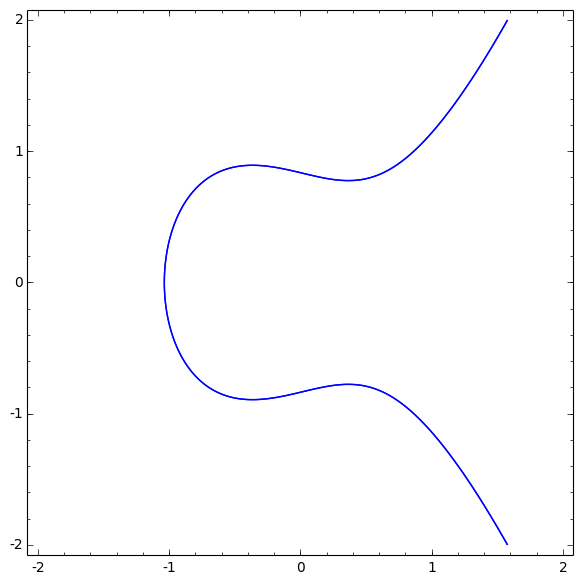
\includegraphics[width=.4\hsize]{weierstrass} & 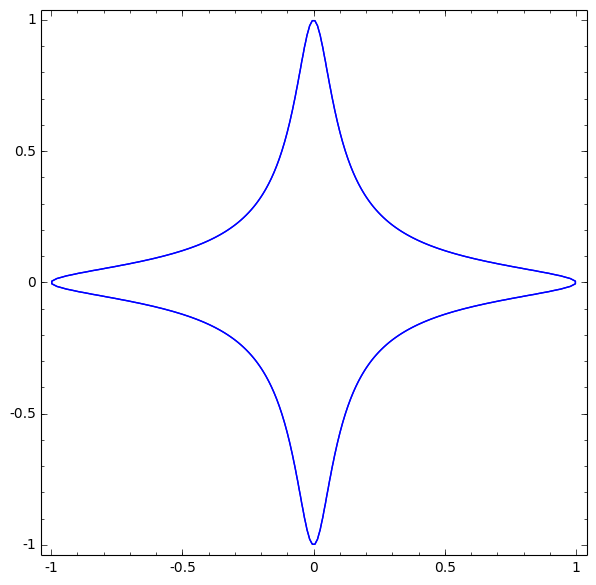
\includegraphics[width=.4\hsize]{edwards} \\
Weierstrass & Edwards \\
\end{tabular}
\end{center}
\end{frame}

\begin{frame}\frametitle{Real zoo (II)}
\begin{center}
\begin{tabular}{cc}
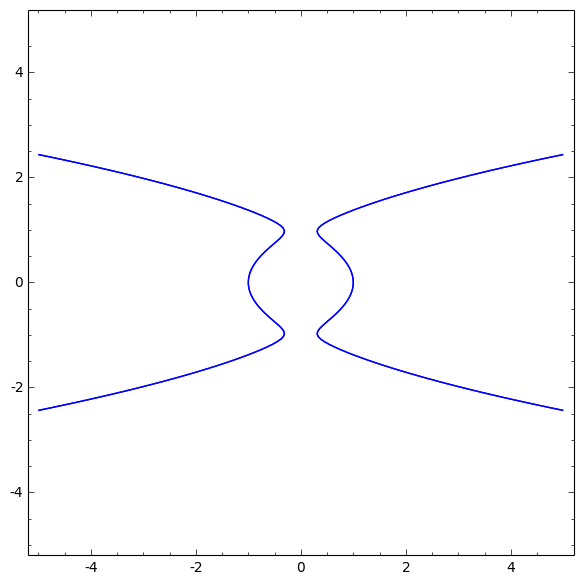
\includegraphics[width=.4\hsize]{jacobi} & 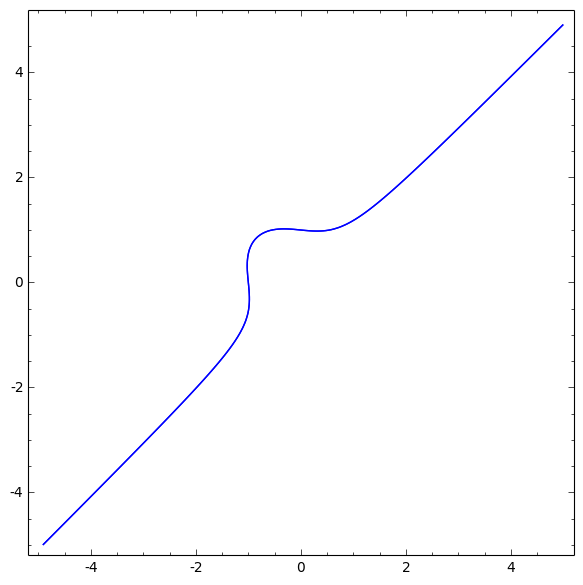
\includegraphics[width=.4\hsize]{hessian} \\
Jacobi & Hess \\
\end{tabular}
\end{center}
\end{frame}

\begin{frame}\frametitle{Finite field zoo}
\begin{center}
\begin{tabular}{cc}
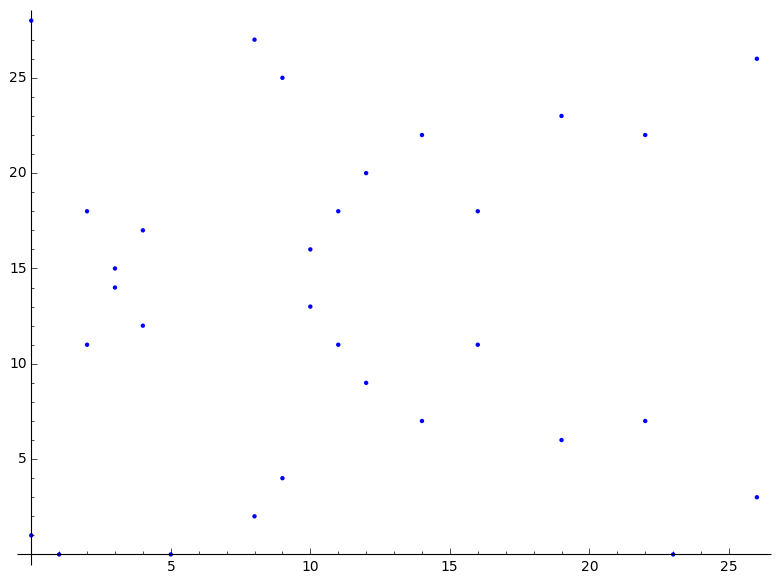
\includegraphics[width=.45\hsize]{frog} & 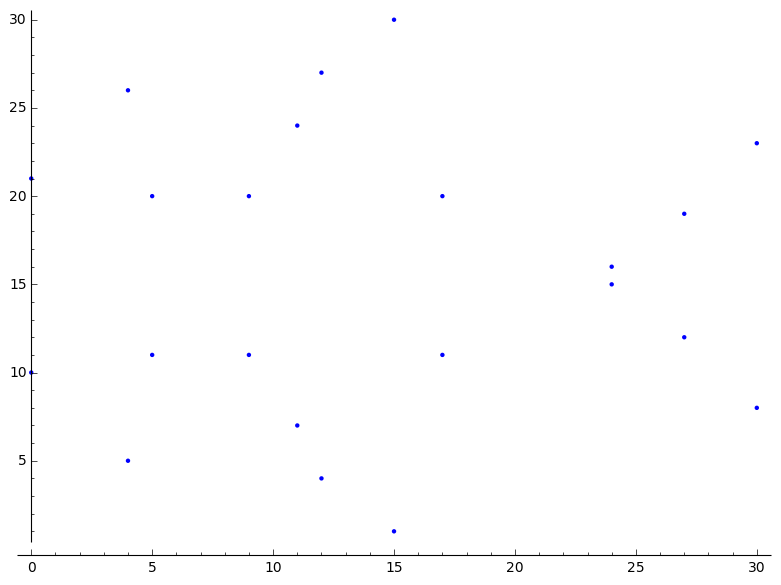
\includegraphics[width=.45\hsize]{cockroach} \\
Frog & Cockroach \\
\end{tabular}
\end{center}
\end{frame}

\begin{frame}\frametitle{Finite field zoo (II)}
\begin{center}
\begin{tabular}{cc}
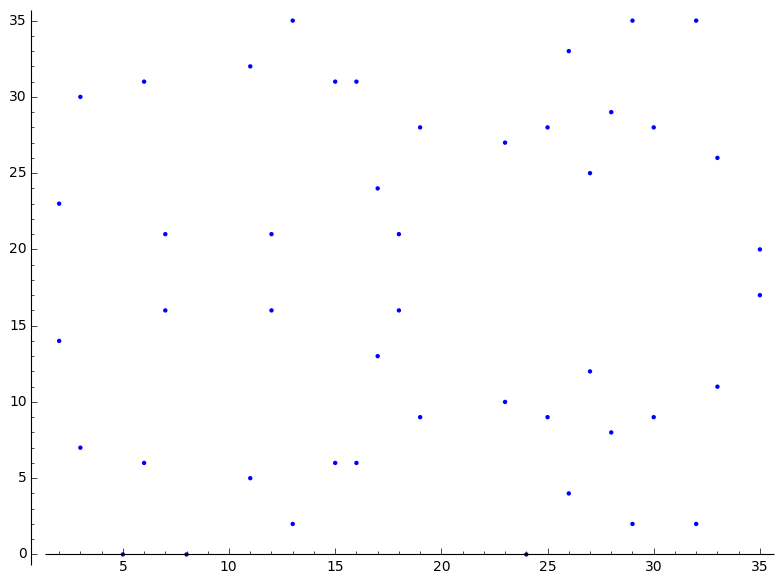
\includegraphics[width=.45\hsize]{walrus} & 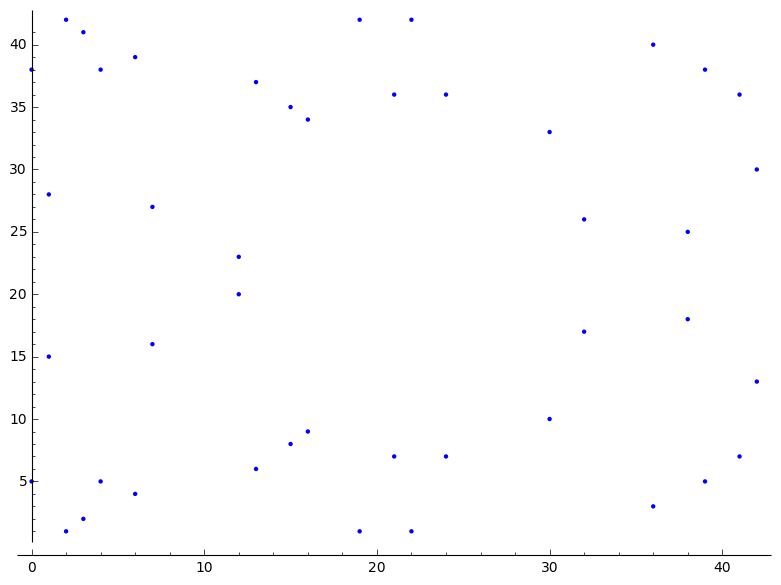
\includegraphics[width=.45\hsize]{bunny} \\
Walrus & Bunny \\
\end{tabular}
\end{center}
\end{frame}

\sectionframe{Transparency}

\subsection{Certificates for elliptic curves}
\begin{frame}\frametitle{Architecture}
\begin{itemize}
\item Provide curves fulfilling a selection of \strong{criteria}\ldots
\item \ldots together with a \imp{certificate} for faster
verification of:
\begin{itemize}
\item the number of points,
\item the discriminant and class number properties,
\item the embedding degree.
\end{itemize}
\bigskip
\item A \strong{deterministic} algorithm to sample curves:
\begin{itemize}
\item Completely \imp{reproducible} generation process.
\item Either pseudo-random (for genericity) or
by enumeration of increasing values (for efficiency).
\item Certify every step,
including \imp{rejected} curves.
\end{itemize}
\end{itemize}
\end{frame}

\begin{frame}\frametitle{Cardinality of curves}
\begin{block}{Prime order}
\begin{itemize}
\item \strong{Certificate}: $(G, q, Π)$
where $G ≠ 0$ is s.t. $q · G = 0$ with $q ≥ p-2√p+1$,
and $Π$~a primality proof for~$q$.
\item \imp{Size} and \imp{verification} in~$O(\log^2 p)$, generally only generated once.
\end{itemize}
\end{block}
\medskip
\begin{block}{Composite order}
\begin{itemize}
\item \strong{Certificate}: $(P, n, c)$,
where $P ≠ 0$ is s.t. $n · P = 0$ with $n < 2 (√p-1)^2$,
and $c$~a composition witness for~$n$.
\item \imp{Size}, \imp{generation} and \imp{verification} in~$O(\log p)$.
\item More efficient \imp{verification} using early-abort SEA information about
small torsion points.
\end{itemize}
\end{block}
\end{frame}

\subsection{Generation process}

\begin{frame}\frametitle{Example}
\begin{itemize}
\item \imp{Sampling function} from the \strong{seed}~$s$:
\begin{itemize}
\item $p$ = smallest prime $≥ s$;
\item $g$ = smallest generator of $\F_p^{×}$;
\item equations of the form $y^2 = x^3 - 3x + b$, $b = g, g^2, …$.
\end{itemize}
\item \imp{Conditions}:
\begin{itemize}
\item $N$ et $N'$ prime;
\item $Δ ≠ 0$, $N, N' ≠ p, p + 1$;
\item embedding degrees of~$E$, $E'$ at least~$p^{1/4}$;
\item class number $≥ p^{1/4}$.
\end{itemize}
\end{itemize}
\end{frame}

\begin{frame}\frametitle{Certificate}
From the seed $s = 2015$: $p = 2017$, $g = 5$,
\begin{block}{\small\tt Curve}\small\tt
(2017, -3, 625)\\
order = 2063, point = (0, 25)\\
twist\_order = 1973\\
disc\_factors = \{6043\}\\
class\_number = 9, form = (17,3,89)\\
embedding\_degree = 1031, factors = \{2, 1031\}\\
twist\_embedding\_degree = 493, factors = \{2, 17, 29\}
\end{block}
\vskip -1.7em
\begin{block}{\small\tt Rejected curves}\small\tt
((2017, -3, 5), composite, 2065, witness, 1679,
  point, (1,258))\\
((2017, -3, 25), torsion\_point, 3, point, (448, 288))\\
((2017, -3, 125), torsion\_point, 2, point, (982, 0))
\end{block}
\end{frame}

\begin{frame}\frametitle{Non-manipulability}
\begin{itemize}
\item Such a process produces \strong{deterministically}
a curve from:
\begin{itemize}
\item a set of \imp{conditions} (including \strong{numerical bounds}),
\item a \imp{sampling function} (including potential \strong{seed}).
\end{itemize}
\item Only a few \imp{conditions} will actually affect the process:
\begin{itemize}
\item twist security,
\item smoothness bounds.
\end{itemize}
\item When a \strong{seed} is needed, suspicion can be avoided:
\begin{itemize}
\item using a \imp{share-commitment} scheme;
\item using \imp{unpredictable} and \imp{unmanipulable} values
(sports results, stock values, lottery results, sunspots, \ldots).
\end{itemize}
\end{itemize}
\end{frame}

\begin{frame}\frametitle{Seed generation}
\begin{center}
%
\includegraphics[width=0.7\hsize]{keyboard_cat}
\animategraphics[loop,autoplay,width=0.7\hsize]{12}{animated_cat/keyboard_cat-}{0}{93}
\end{center}
\end{frame}

\begin{frame}\frametitle{Questions?}
\begin{center}
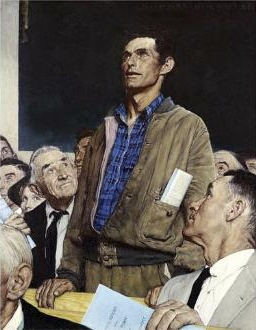
\includegraphics[width=.45\hsize]{rockwell_speech}
\end{center}
\end{frame}
\end{document}
